\documentclass[conference]{IEEEtran}

\usepackage{amsmath, amsthm, amssymb, dsfont, accents}

\usepackage{tikz,pgfplots}
\usepackage{hyperref, booktabs}
\usepackage{biblatex}
\usepackage{todonotes}

\pgfplotsset{compat=1.14}

\usetikzlibrary{calc, automata}
\newlength\figureheight
\newlength\figurewidth

\addbibresource{2_references.bib}

\pdfinfo{
   /Author (Homer Simpson)
   /Title  (Robots: Our new overlords)
   /CreationDate (D:20101201120000)
   /Subject (Robots)
   /Keywords (Robots;Overlords)
}

% MDPs
\newcommand{\MDP}{\mathbb{M}}

\newcommand{\X}{\mathbb{X}}
\newcommand{\U}{\mathbb{U}}
\newcommand{\init}{\rho}
\newcommand{\tr}{T}

\newcommand{\pol}{\mu}

% LTL
\newcommand{\True}{\texttt{true}}
\newcommand{\False}{\texttt{false}}
\newcommand{\AP}{AP}

\newcommand{\ltluntil}{\mathcal{U}}
\newcommand{\ltlnext}{\bigcirc}

\newcommand{\alphabet}{{2^{\AP}}}
\newcommand{\word}{\boldsymbol{\pi}}
\newcommand{\letter}{\pi}
\newcommand{\lab}{L}

\newcommand{\FSA}{\mathcal{A}}

% Probability
\newcommand{\Prob}{\mathbf{P}}


% Value iteration
\newcommand{\bellman}{\mathcal{B}}


% Math
\DeclareMathOperator*{\argmin}{arg\,min}
\DeclareMathOperator*{\argmax}{arg\,max}
\newcommand{\ind}{\mathbf{1}}


\newtheorem{problem}{Problem}
\newtheorem{theorem}{Theorem}
\newtheorem{definition}{Definition}
\newtheorem{remark}{Remark}
\newtheorem{example}{Example}

\newcommand{\red}[1]{{\color{red} #1 }}
\newcommand{\sofie}[1]{{\color{orange}#1}}
\newcommand{\sofieNew}[1]{{\color{blue}#1}}
\begin{document}

%\title{\huge Sequential Value Iteration for Modular Systems Applied to Collaborative Space Robotics}

%\title{\huge Specification-oriented Active Exploration via Sequential Dynamic Programming: Applications to Space Exploration via a Rover-Copter Team}

%\title{\huge Specification-guided Active Exploration: Applications to Safety-critical Mars Rover-Copter Mission}

\title{\huge Specification-guided Active Exploration: Applications to a Risk-averse Rover/Copter Mars Mission}

%\title{\huge Verifiability-oriented Active Exploration: Applications to Safety-critical Mars Rover-Copter Team}

%\title{\huge Satisfaction-oriented Active Exploration: Applications to Safety-critical Mars Rover-Copter Team}

\author{Anonymous submission}

\maketitle

\begin{abstract}
  As a step towards achieving autonomy in space exploration missions we consider a collaborative robotics system with a copter and a rover. The goal of the copter is to explore an unknown environment so as to maximize the probability that the rover can satisfy a science mission expressed in Linear Temporal Logic. We formulate the problem as a two-step dynamic program and mitigate the curse of dimensionality for this large system by leveraging its decomposed nature. We demonstrate in simulations and on hardware that the robot team makes intelligent decisions in the face of uncertainty.
\end{abstract}

\IEEEpeerreviewmaketitle

	
%%%%%%%%%%%%%%%%%%%%%%%%%%%%%%%%%%%%%%%%%%%%%%%%
%%%%%%%%%%%%%%%%%%%%%%%%%%%%%%%%%%%%%%%%%%%%%%%%

\section{Introduction}

Environment exploration and task planning are crucial components of any autonomous system. In most approaches, these two aspects are decoupled in the sense that exploration is performed to maximize knowledge overall, rather than to maximize knowledge \emph{pertaining to the task}. In this work, we aim to improve efficiency in situations where exploration is expensive by limiting exploration to areas crucial for accomplishing a given task. 

Due to the growing complexity and uncertainty in future space missions, autonomy is a crucial ability for missions' success. In this work, we will focus on multi-asset missions (team of robots), in particular the 2020 Mars mission that will consist of a ground rover and a copter for exploration (Fig. \ref{fig:heli-rover}). To increase productivity and science return, the robotic team needs to autonomously perform multi-sol (sol: martian day) navigation without human intervention. Severe communication delays and resource constraints (like battery time and limited hours of sunlight) pose further challenges in achieving such autonomy. In these missions, partial knowledge about the environment is typically available from satellite imagery, but it needs to be complemented with observations from on-board sensors. Our goal is to improve both autonomy and efficiency in such missions by developing principled methods that in a specification-guided manner determine the most important areas to explore. 

Our approach lies at the intersection of formal synthesis methods and stochastic optimal control: we phrase the exploration problem as a two-stage optimal control problem in the combined space of copter poses and environment beliefs.
To partially circumvent the curse of dimensionality in the resulting large system we leverage its decomposed nature and perform value iteration via sequential back stepping, which avoids construction of the overall system.

\todo[inline]{Cristi/Ali: Short review of state-of-the-art mapping methods; active exploration; other related work}

vision-based planning-oriented mapping...
confidence-rich mapping...
but these methods typcally do not consider specificaitons and cannot handle constraints...

Three principal methods exist to solve stochastic optimal control problems: value iteration, policy iteration, and linear programming \cite{Bertsekas1978}. Approximate solutions methods to the stochastic optimal control problem under temporal logic constraints have been proposed via parametrized value function approximations \cite{Papusha2016,Leong2016}, and via tensor decompositions \cite{Alora2016}. While the above mentioned approaches are general in scope, we focus on uncertainty stemming from an unknown environment which we model in a way that leads to a naturally decomposed problem. 

% Unfortunately, in practice all three methods are limited to finite-state systems of moderate size. For systems with continuous state spaces, or systems that are very large, approaches include approximate dynamic programming (also known as reinforcement learning) \cite{Powell2011} and abstraction-based methods \cite{Zamani2015,Haesaert2017}. Approximate solutions methods to the stochastic optimal control problem under temporal logic constraints have been proposed via parametrized value function approximations \cite{Papusha2016,Leong2016}, and via tensor decompositions \cite{Alora2016}. While the above mentioned approaches are general in scope, we focus on uncertainty stemming from an unknown environment which we model in a way that leads to a naturally decomposed problem. 


\begin{figure}
  \begin{center}
    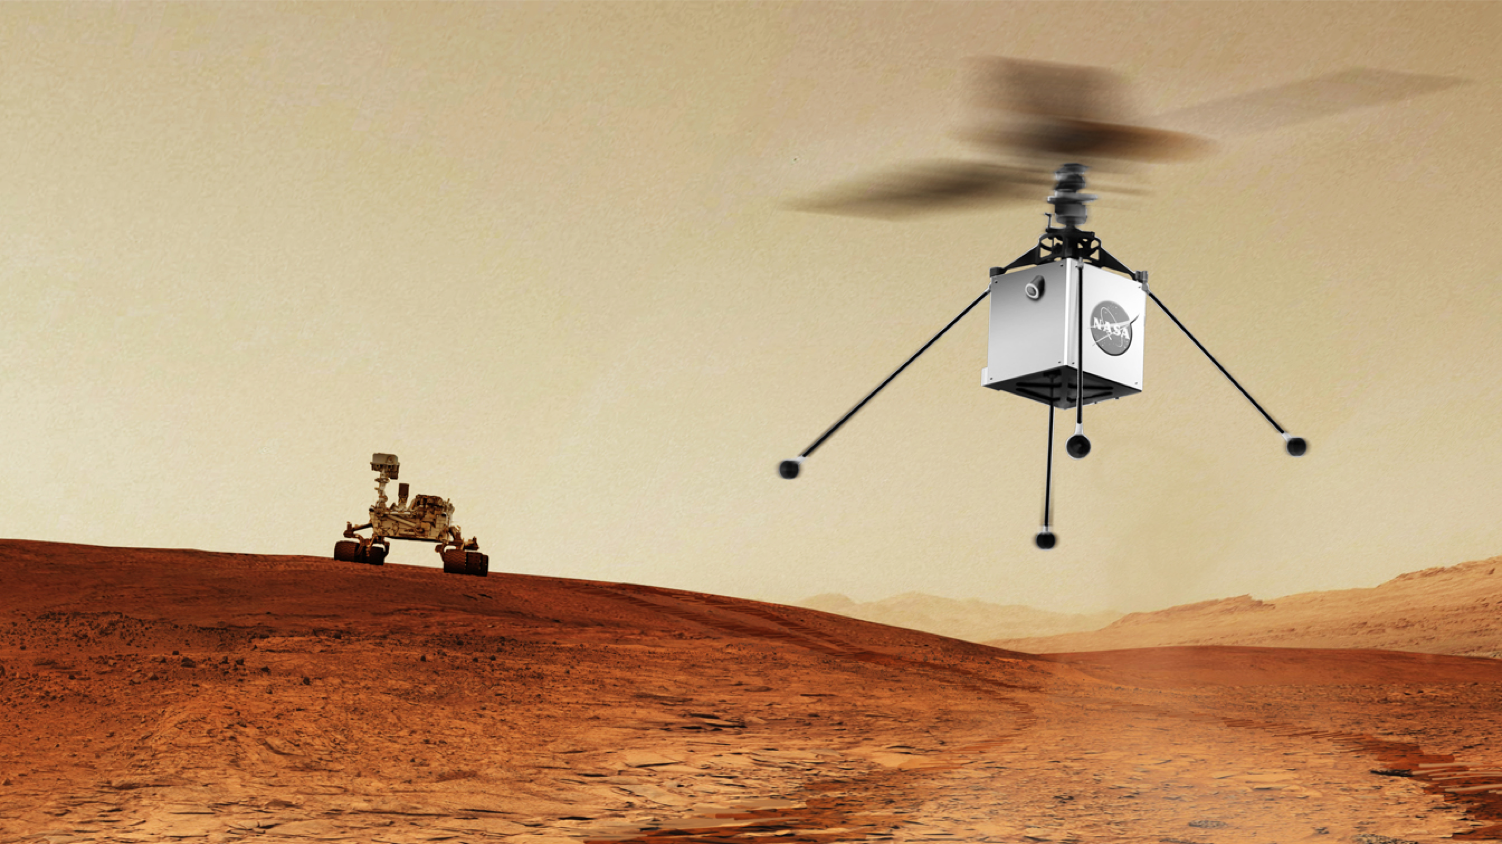
\includegraphics[width=0.8\columnwidth]{figs/heli-rover.png}
  \end{center}
  \caption{Cooperative robotics team for Mars exploration.}
  \label{fig:heli-rover}
\end{figure}

\subsection{Paper layout}

% The following Section \ref{sec:preliminaries} introduces pertinent notation along with basics of probabilistic systems and temporal logics. Subsequently, Section \ref{sec:problem} introduces the problem we seek to solve, followed by our proposed solution in Section \ref{sec:solution}. We demonstrate the approach in a Mars-inspired case study in Section \ref{sec:casestudy}, and report our experience from hardware experiments in Section \ref{sec:hardware}. The paper is concluded in Section \ref{sec:conclusion}.


\section{Problem Setup}
\label{sec:problem}

In this section, we will go over the two-robot scenario .... of reaching goal... satisfying some specification...

We will start by modeling the decision making process in its most general form as an MDP... Then, we will discuss how the map uncertainty is modeled.... and defined concrete specifications in and resource-constraints/requirements, ....

Objectives of this work is threefold: 1) compute ..., 2) analyze ..., 3) develop ...

\subsection{Modeling}

All systems in this paper are modeled as Markov Decision Processes, or as combinations (products) of MDPs. An MDP is defined as follows \cite{Bertsekas1978}:

\begin{definition}
\label{def:MDP}
  A discrete-time \textbf{Markov decision process} (MDP) is a tuple $\MDP = (\X, \init, \tr, \U)$ where
  \begin{itemize}
    \item $\X$ is a state space with states $x\in\X$; % as its elements;
    \item $\rho \in \mathcal P (\X)$ is an initial distribution;
    \item $\U$ is a input space with inputs $u\in\U$;
    \item $\tr$ is a conditional stochastic kernel that assigns to each state $x\in \X$ and control $u\in \U$ a probability distribution $\tr(\cdot\mid x,u)$ over $\X$.
  \end{itemize}
\end{definition}

An \emph{execution} of $\MDP$ is a state-input sequence $(x_0, u_0)(x_1, u_1)\ldots$ where $x_0 \sim \rho$ and $x_{k+1} \sim \tr(\cdot \mid x_k, u_k)$ for inputs $u_k \in \U$. A \emph{policy} $\pol = \pol_0 \pol_1 \ldots$ is a sequence of conditional probability distributions $\pol_k( \cdot \mid x_0, \ldots, x_{k})$. We say that a policy is \emph{Markov} if $\pol_k( \cdot \mid x_0, \ldots, x_{k}) = \pol_k( \cdot \mid x_{k})$ for all $k$. If a trajectory $(x_0, u_0)(x_1, u_1)\ldots$ is such that $u_k \sim \pol_k ( \cdot \mid x_{k})$ we say that the trajectory is \emph{generated} by $\pol$.


\subsection{Environment uncertainty as a belief MDP}

A common way to represent a map for planning purposes is to attach labels such as ``sand'' or ``rock'' to different locations, but in a Mars setting the true labels are often only partially known at the time of system deployment. We capture this environmental uncertainty with MDPs $\MDP_{e_i}$ that model belief dynamics over labels. Transitions in the MDPs occur when measurements are taken from on-board sensors, i.e. the robots need to be physically close to a region to obtain information about its true labels. 

\todo[inline]{Example of belief MDP}

Belief MDPs can then be combined with models of robots that can move around and take measurements. In an uncertain environment satisfaction of a given specification is a function of the true environment, and thus stochastic. Our objective is to extract control policies that maximize the knowledge about the satisfiability of a given task: either we want the exploration to show that the task can be completed with a high probability, or that the probability of task completion is very low. Both are desirable outcomes since a negative results allows resources to be redirected towards more realistic objectives.  

\subsection{Specifications}

The basic building blocks of specifications are \emph{atomic propositions} that take values $\True$ or $\False$. An atomic proposition $p$ is associated with a subset $A$ of a state space $\X$ in the sense that $p = \True$ if and only if $x \in A$. By combining atomic propositions into a formula, desired system behavior is expressed as set membership constraints (atomic propositions) together with temporal relations (operators).

Consider a set $AP = \{ p_1, \ldots, p_L \}$ of atomic propositions; it defines an \emph{alphabet} $\alphabet$ where each \emph{letter} $\letter$ of the alphabet is defined as a set of atomic propositions. An infinite string of letters is a \emph{word} $\word=\letter_0\letter_1\letter_2\ldots$%\in\alphabet^{\mathbb{N}}$
, which should be thought of as the observed output of a system. \todo{\tiny removed $\alphabet^{\mathbb{N}}$ as it doesnt seem correct. }
\sofieNew{More specifically for each execution of the MDP system,  $\mathbf{x} = x_0 x_1 x_2 \ldots$ , we use the }
%To quantify the dynamic behavior of a system, we define the word associated to an MDP execution. Consider a 
labeling function $\lab: \X \rightarrow \alphabet$ to 
associate the word $\word = \lab(x_0)\lab(x_1) \lab(x_2) \ldots$. Thus for each time instance $i$, $L(x_i)$ maps the current state $x_i$ to a letter in the alphabet $\alphabet$.
%The words generated by a state trajectory $\mathbf{x} = x_0 x_1 x_2 \ldots$ can be defined as the word $\word = \lab(x_0)\lab(x_1) \lab(x_2) \ldots$.
\sofieNew{Desired behavioral properties can now be expressed via temporal logic formulas over the generated words.}
%\red{System properties can now be expressed via temporal logic formulas over the generated words. [not fully true]}
%Properties are formulas composed of atomic propositions and operators. 
In the sequel we focus on a fragment of linear temporal logic. 
\begin{definition}
  \label{def:gdtl-syntax}
  Formulas in the \textbf{syntactically co-safe LTL} (scLTL) fragment are constructed according to the grammar
  \begin{equation*}
    \label{eq:scLTL}
    \psi ::=  \True \ |\ p \ |\ \lnot p \ |\ \psi_1 \vee\psi_2  \ |\ \psi_1 \land \psi_2 \ |\ \psi_1 \ltluntil \psi_2 \ |\ \ltlnext \psi,
  \end{equation*}
  where $p\in \AP$ is an atomic proposition.
\end{definition}
% The syntax defines the symbols and their correct ordering to form a formulae.
An advantage of considering the scLTL fragment is that policy synthesis for a scLTL specification over a space $\X$ is equivalent to reachability of $\X\times Q_f$ on the product system $\MDP \otimes_{ser} \FSA_\psi$, where $\FSA_\varphi$ is a finite-state automaton constructed from $\varphi$ \cite{Belta2017} with accepting set $Q_f$. A finite-state automaton is a special case of an MDP, thus also the product system is an MDP. It is well known that the optimal reachability probability can be computed via value iteration of a Bellman operator \cite{Baier2008}. To define the interpretation of a formula, i.e. the \emph{semantics}, consider a word $\word$.

\begin{definition}
 The \textbf{semantics} of scLTL are defined recursively as follows: $\word$ \textbf{satisfies} $\psi$ at time $k$, written $(\word, k) \models \psi$, if
 \begin{itemize}
    \item $(\word, k) \models \True$;
    \item $(\word, k) \models p$ iff $p \in \letter_k$;
    \item $(\word, k) \models \psi_1 \land  \psi_2  $ iff $ ( (\word, k) \models \psi_1 ) \land ( (\word, k) \models \psi_2 ) $;
    \item $(\word, k) \models \psi_1 \lor  \psi_2  $ iff $ ( (\word, k) \models \psi_1 ) \lor ( (\word, k) \models \psi_2 ) $;
    \item $(\word, k) \models  \psi_1 \ltluntil \psi_2 $ iff $\exists j \geq k \text{ s.t. } ((\word, j) \models \psi_2 ) $ and $(\word, l) \models \psi_1, \forall l \in \{k, \ldots j-1\}$;
    \item $(\word, k) \models \ltlnext \psi$ iff $(\word, k+1) \models \psi$.
 \end{itemize}

\end{definition}

We say that a state trajectory $\mathbf{x} = x_0 x_1 x_2 \ldots$ satisfies a specification $\psi$, written $\mathbf{x} \models \psi$, if the generated word $\word =\lab(x_0) \lab(x_1) \lab(x_2) \ldots$ satisfies $\psi$ at time 0, i.e. $\word_0 \models \psi$.

\sofieNew{In general, we cannot say that an MDP system (for a given policy) satisfies a property $\psi$. Instead, we can quantify the probability with which the system will satisfy the property, that is  \[\mathbb P[\mathbf x \vDash \psi ] .\]
}


\todo[inline]{Example of a specification in rover and environment belief}

\subsection{Two-stage Execution}
%
%\begin{figure}
%	\begin{center}
%		\begin{tikzpicture}
%			\draw[|-|] (0,0) node[yshift=-1mm, anchor=north] {$0$} -- (3,0) node[yshift=-1mm, anchor=north] {$T_c$};
%			\draw[|-|] (3,0) -- (6,0) node[xshift=3mm, yshift=-1mm, anchor=north] {$T_c + T_r$};
%			\draw[|-latex] (6,0) -- (7,0) node[anchor=west] {$t$};
%
%			\node at (0,0.3) {$x_c$};
%			\node at (0,0.6) {$x_e$};
%
%			\node at (3,0.3) {$x_c$};
%			\node at (3,0.6) {$x_e$};
%			\node at (3,0.9) {$x_r$};
%
%			\node at (6,0.6) {$x_e$};
%			\node at (6,0.9) {$x_r$};
%
%			\draw[-latex] (0.5,0.3) -- (2.5,0.3);
%			\draw[-latex] (0.4,0.6) -- (2.5,0.6);
%
%			\draw[-latex] (3.5,0.9) -- (5.5,0.9);
%			\draw[-latex] (3.5,0.6) -- (5.5,0.6);
%
%			\node (expl) at (1.5, -0.5) {Exploration};
%			\node (miss) at (4.5, -0.5) {Mission};
%
%			\draw[dashed] (0,0) -- ($(expl.west)$);
%			\draw[dashed] (3,0) -- ($(expl.east)$);
%
%			\draw[dashed] (3,0) -- ($(miss.west)$);
%			\draw[dashed] (6,0) -- ($(miss.east)$);
%
%		\end{tikzpicture}
%	\end{center}
%	\caption{Illustration of execution order. In the exploration phase $[0, T_c]$ the copter explores the environment, whereas the rover executes the scientific mission on $[T_c, T_c + T_r]$.}
%	\label{fig:execorder}
%\end{figure}

\begin{figure}
	
\centering	
	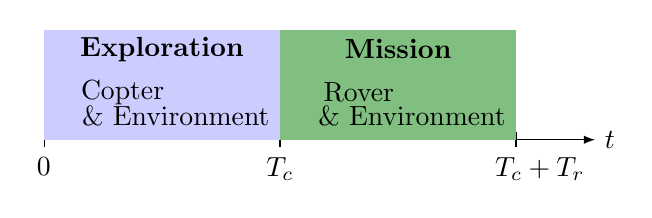
\begin{tikzpicture}
			\draw[|-|] (0,0) node[yshift=-1mm, anchor=north] {$0$} -- (3,0) node[yshift=-1mm, anchor=north] {$T_c$};
			\draw[|-|] (3,0) -- (6,0) node[xshift=3mm, yshift=-1mm, anchor=north] {$T_c + T_r$};
			\draw[|-latex] (6,0) -- (7,0) node[anchor=west] {$t$};
			\fill[color=blue!20]  (0,0) -- (3,0) -- (3,1.4) -- (0,1.4)--cycle;
				\fill[color=green!50!black!50]  (3,0) -- (6,0) -- (6,1.4) -- (3,1.4)--cycle;

%			\node at (0,0.3) {$x_c$};
%			\node at (0,0.6) {$x_e$};
			\node at (1.5,0.3) {\ \ \ \& Environment};
			\node at (4.5,0.3) {\ \ \ \& Environment};
			\node at (1,0.6) {Copter};
			\node at (4,0.6) {Rover};
%			\node at (3,0.3) {$x_c$};
%			\node at (3,0.6) {$x_e$};
%			\node at (3,0.9) {$x_r$};
%
%			\node at (6,0.6) {$x_e$};
%			\node at (6,0.9) {$x_r$};

%			\draw[-latex] (0.5,0.3) -- (2.5,0.3);
%			\draw[-latex] (0.4,0.6) -- (2.5,0.6);
%
%			\draw[-latex] (3.5,0.9) -- (5.5,0.9);
%			\draw[-latex] (3.5,0.6) -- (5.5,0.6);
		
			
			\node (expl) at (1.5, 1.15) {\bfseries \color{black} Exploration};
			\node (miss) at (4.5, 1.15) {\bfseries \color{black} Mission};

%			\draw[dashed] (0,0) -- ($(expl.west)$);
%			\draw[dashed] (3,0) -- ($(expl.east)$);
%
%			\draw[dashed] (3,0) -- ($(miss.west)$);
%			\draw[dashed] (6,0) -- ($(miss.east)$);

		\end{tikzpicture} 
			\caption{Illustration of execution order. In the exploration phase $[0, T_c]$ the copter explores the environment, whereas the rover executes the scientific mission on $[T_c, T_c + T_r]$.}	\label{fig:execorder}
\end{figure}

We consider a system consisting of the following components:
\begin{enumerate}
	\item An MDP $\MDP_{rov}$ with state $x_r$ modeling a ground rover in 2D space.
	\item An MDP $\MDP_{env}$ with state $x_e$ that captures belief dynamics over a collection of unknown environment labels.
	\item A scLTL specification $\varphi$ that expresses the requirement of the scientific mission. The formula is defined over a set of atomic propositions in $\X_{rov} \times \X_{env}$---the combined space of rover poses and environment beliefs. 
	\item An MDP $\MDP_{copt}$ modeling a copter in 3D space.
	\item A measurement model that dictates how the state of $\MDP_{env}$ is updated from measurements received from the rover and copter. For instance, it is reasonable to assume that the rover can take measurements of a given region provided that it is sufficiently close, and that the copter can take measurements of regions it flies above. Copter measurements also depend on the altitude: a high-flying copter can see a larger area but the image resolution is better if the copter is close to the ground.    
\end{enumerate}

Due to the nature of the problem (the copter is quick and has short battery life, the rover is slow), it is reasonable to consider a turn-based solution.
\sofie{[solution to which problem?]}
 We therefore propose to solve the problem sequentially by dividing it into two phases: exploration and mission execution. As shown in Fig. \ref{fig:execorder}, the copter is active in the exploration phase, whereas the rover conducts the scientific mission in the second phase. We assume that the exploration phase lasts for a time $T_c$, and that the mission phase lasts at most for a time $T_r$. These times can be informed e.g. by available battery capacity and remaining hours of daylight. In both phases the environment belief is updated according to measurements taken by the copter and rover. We can now state the question we attempt to answer in this paper.
\begin{problem}
\label{prob:main}
  Consider the model components listed above. Design a policy for the copter exploration phase that explores the environment in a way that maximizes the expected knowledge about satisfaction of the scientific mission at time $T_c$.
\end{problem}

In the rest of the paper we will assume that all MDPs are finite, i.e. they have finite state and input spaces. To handle continuous-state MDPs, there are principled methods to construct finite-state approximations and relate finite solutions to the original problem \cite{Zamani2015,Haesaert2017}. An alternative is to use approximate dynamic programming (also known as reinforcement learning) \sofie{[ADP is not equal to RL. ADP is model-based, whereas RL is model-free.]} directly on the continuous state space \cite{Powell2011}. Approximate methods allow a trade-off between the degree of approximation and scalability.\sofie{[This is for standard dynamic programming, most of the bounds require some type of contractivity (enforced by the discounting.)]}


\section{Product MDPs and Value Iteration}

\begin{figure}
\begin{center}
    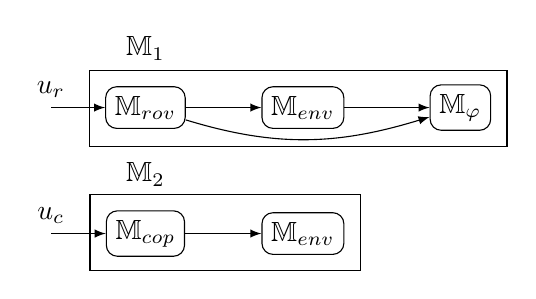
\begin{tikzpicture}
    \node[draw, node distance=2cm, rounded corners] (rover) {$\MDP_{rov}$};
    \node[draw, node distance=2cm, rounded corners, right of=rover] (environment) {$\MDP_{env}$};
    \node[draw, node distance=2cm, rounded corners, right of=environment] (fsa) {$\MDP_\varphi$};

    \draw[-latex] (rover) --  (environment);
    \draw[-latex] (environment) --  (fsa);
    \draw[-latex] (rover) to[out=-17, in=197] (fsa);

    \draw ([xshift=-2mm, yshift=2mm]$(rover.north west)$) rectangle ([xshift=2mm, yshift=-2mm]$(fsa.south east)$) {};
    \node[above of=rover, node distance=0.75cm] {$\MDP_1$};

    \draw[latex-] (rover) -- ++(-1.2,0) node[coordinate] (west) {} node[above] {$u_r$};

    \node[below of=rover, draw, node distance=1.6cm, rounded corners] (copter) {$\MDP_{cop}$};
    \node[draw, node distance=2cm, rounded corners, right of=copter] (env2) {$\MDP_{env}$};

    \draw[-latex] (copter) --  (env2);

    \draw ([xshift=-2mm, yshift=2mm]$(copter.north west)$) rectangle ([xshift=2mm, yshift=-2mm]$(env2.south east)$) {};
    \node[above of=copter, node distance=0.75cm] {$\MDP_2$};

    \draw[latex-] (copter) -- ++(-1.2,0) node[coordinate] (west) {} node[above] {$u_c$};

  \end{tikzpicture}
\end{center}
  \caption{Illustration of aggregate systems $\MDP_1$ and $\MDP_2$ constructed as serial products, where $\MDP_{env}$ is itself a parallel product.}
  \label{fig:agg}
\end{figure}


\subsection{Product MDPs}
\label{sub:products}

We convert the specification $\varphi$ into a deterministic finite automaton $\MDP_\varphi$---a special case of a MDP. In the exploration phase the copter and environment systems are active; whereas in the mission phase the aggregate system consists of the rover, the environment, and the specification automaton. The two aggregate systems $\MDP_1$ and $\MDP_2$ are illustrated in Fig. \ref{fig:agg}. Our solution relies on value iteration performed on these aggregate systems. Value iteration can be an expensive operation: it requires knowledge of the transition probabilities between any two aggregate states. However, the aggregate systems we consider are composed of different parts: robots, environment belief and specification automaton. In addition, the environment belief MDP itself is composed of several belief MDPs over individual labels. Here we generalize these types of compositions and show below how value iteration can be performed without having to construct the aggregate systems explicitly. First we define two types of canonical compositions of MDPs $\MDP_1 = (\X_1, \init_1, \U_1, \tr_1)$ and $\MDP_2 = (\X_2, \init_2, \U_2, \tr_2)$: serial and parallel products.
\begin{definition}
  The \textbf{parallel product} of $\MDP_1$ and $\MDP_2$ is the MDP $\MDP_1 \otimes_{par} \MDP_2 = (\X_1 \times \X_2, \init_{par}, \U_1 \times \U_2, \tr_{par})$, where $\init_{par}(x_1, x_2) = \init_1(x_1) \init_2(x_2)$
  and
  \begin{equation}
  \begin{aligned}
      \tr_{par}&(x_1', x_2' \mid x_1, x_2, u_1, u_2) \\
      & = \tr_1 (x_1' \mid x_1, u_1) \tr_2 (x_2' \mid x_2, u_2)
  \end{aligned}
  \end{equation}
\end{definition}

\begin{definition}
  Given a \textbf{connection} $C : \X_1 \rightarrow \U_2$, the \textbf{serial product} of $\MDP_1$ and $\MDP_2$ is the MDP $\MDP_1 \otimes_{ser}^C \MDP_2 = (\X_1 \times \X_2, \init_{ser}, \U_1, \tr_{ser})$,
  where $\init_{ser}(x_1, x_2) = \init_1(x_1) \init_2(x_2)$
  and
  \begin{equation}\label{eq:serial}
  \begin{aligned}
      \tr_{ser}&(x_1', x_2' \mid x_1, x_2, u_1) \\
      & = \tr_1 (x_1' \mid x_1, u_1) \tr_2 (x_2' \mid x_2, C(x_1') )
  \end{aligned}
  \end{equation}
\end{definition}
In a parallel product there is no interaction between the two MDPs, but in a serial product a transition $x_1 \rightarrow x_1'$ in $\MDP_1$ triggers an action $C(x_1')$ in $\MDP_2$ that results in a transition in $x_2' \sim T_2(\cdot \mid x_2, C(x_1'))$. Both products can be generalized to more than two components, and products can also be nested: e.g. $\MDP_1 \otimes_{ser}^C \left( \MDP_2 \otimes_{par} \MDP_3 \right)$. Large nested products lead to large state spaces, and since the size of the transition matrix is quadratic in the size of the state space, computation of the aggregate transition matrix quickly becomes challenging. However, we next show that value iteration can be done sequentially over subsystems without computing the aggregate transition matrices.

With these definitions we can write the aggregate systems $\MDP_1$ and $\MDP_2$ as:
\begin{equation}
\label{eq:syst_prod_def}
\begin{aligned}
	\MDP_1 & = \left( \MDP_{rov} \otimes_{ser}^{C_1} \left( \MDP_{e_1} \otimes_{par} \ldots \otimes_{par} \MDP_{e_n} \right) \right) \otimes_{ser}^{C_2} \mathcal A_{\varphi}, \\
	\MDP_2 & = \MDP_{cop} \otimes_{ser}^{C_3} \left( \MDP_{e_1} \otimes_{par} \ldots \otimes_{par} \MDP_{e_n} \right),
\end{aligned}
\end{equation}
where $\MDP_{e_i}$ is the $i$th uncertain environment label. The connections $C_1$, $C_2$ and $C_3$ represent the following mappings:
\begin{itemize}
	\item $C_1 : \X_{rov} \rightarrow \U_{e_1} \times \ldots \times \U_{e_n}$ and $C_3 : \X_{cop} \rightarrow \U_{e_1} \times \ldots \times \U_{e_n}$ map poses of the rover and copter to measurements of the environment labels,
	\item $C_2 : \X_{rov} \otimes \X_{env} \rightarrow \U_{\varphi}$ maps the joint space of rover poses and environment belief states to $2^{AP}$, where $AP$ is the set of atomic propositions used to construct $\varphi$.
\end{itemize}
We now turn to value iteration for this type of product system.

\subsection{Value Iteration for Product MDPs}
\label{sub:valueit}

Given a function $g: \X \times \mathbb{R}_+ \rightarrow \mathbb{R}_+$, consider a general Bellman operator $\bellman : (\X \rightarrow \mathbb{R}_+) \rightarrow (\X \rightarrow \mathbb{R}_+)$ on the following form:
\begin{equation}
  (\bellman V) (x) = \sum_{x' \in \X} \max_{u \in \U} g(x', V(x')) T(x' \mid x, u).
\end{equation}

If $\mathbf{\Pi}$ is the set of all stationary policies, the optimal value function $V^*$ and policy $\pol^*$ for a given bellman operator $\bellman$ is then found via the iterations

\begin{subequations}
\label{eq:value_iter}
  \begin{align}
    & V^*_0 \equiv 0, \\
    & V^*_{k+1}  = \bellman V_k \label{eq:iter}, \\
    & \pol^* \in \argmax_{\pol \in \mathbf{\Pi}} \sum_{x' \in \X}  g(x', V^*(x')) T(x' \mid x, \pol(x)).
  \end{align}
\end{subequations}

\begin{example}
  For the Bellman operator corresponding to reaching a set $X_f$, the function $g$ is given by
  \begin{equation}
  \label{eq:bellman_reach}
    g(x', v') = \max( \ind_{X_f}(x'), v').
  \end{equation}
  This is exactly the operator needed to compute the value functions \eqref{eq:rovervalue} and \eqref{eq:coptervalue} \cite{Abate2008}.
\end{example}

\begin{example}
  Consider the finite-horizon optimal control problem 
  \begin{equation}
     \max \sum_{t=0}^T J_t(x_t).
  \end{equation} 
  In this case, if the dynamic programming is initialized with $V_T(x) = J_T(x)$, iterated applications of the Bellman operator corresponding to $g_t(x', v') = J_{t-1}(x') + v'$, i.e.
  \begin{equation*}
    V_{t-1}(x) = \bellman_t V_{t} (x) = \max_{\pol} (J_{t-1}(x') + V_{t}(x')) T(x' \mid x, \pol(x))
  \end{equation*}
  computes the value function at times $T-1, T-2, \ldots, 0$.
\end{example}

We now consider the Bellman iteration step for product MDPs. For a serial product we get
\begin{equation*}
\begin{aligned}
  & \bellman V (x_1, x_2) = \hspace{-5mm} \sum_{x_1', x_2' \in \X_1 \times \X_2} \max_{u_1 \in \U_1} \left[ \begin{aligned}
  	g(x_1', x_2', V(x_1', x_2')) \\
  	\times T_{ser}(x_1', x_2' \mid x_1, x_2, u_1)
  \end{aligned} \right] \\
  & = \sum_{x_1' \in \X_1} \max_{u_1 \in \U_1} T_1(x_1' \mid x_1, u_1 ) \left[ \begin{aligned}
   	\sum_{x_2' \in \X_2}  g(x_1', x_2', V(x_1', x_2')) \\
   	\times  T_2(x_2' \mid x_2, C(x_1'))
   \end{aligned} \right].
\end{aligned}
\end{equation*}
It follows that the Bellman update $V \mapsto \bellman V$ for a serial product can be computed in back-stepping fashion as follows:
\begin{equation*}
\begin{aligned}
  W_2(x_1', x_2') & = g(x_1', x_2', V(x_1', x_2')) \\
  W_1(x_1', x_2) & = \sum_{x_2' \in \X_2}  T_2(x_2' \mid x_2, C(x_1')) W_2(x_1', x_2'), \\
  \bellman V(x_1, x_2) & = \sum_{x_1' \in \X_1} \max_{u_1 \in \U_1} T_1(x_1' \mid x_1, u_1) W_1(x_1', x_2).
\end{aligned}
\end{equation*}
The procedure generalizes immediately to $n$-length serial products and steps
\begin{equation}
\label{eq:general_decomp}
\begin{aligned}
  & W_{i-1}(x_1', \ldots, x_{i-1}', x_i, \ldots, x_n) \\
  & \quad = \sum_{x_{i}' \in \X_{i}} \left[ \begin{aligned} & T_{i} (x_{i}' \mid x_{i}, C(x_{i-1}')) \\ 
   & \times W_{i} (x_1', \ldots, x_{i-1}', x_i', \ldots, x_n)
    \end{aligned} \right].
\end{aligned}
\end{equation}

\begin{remark}
  In serial products of arbitrary length a connection $C_i$ can be defined either as $C_i: \X_{i-1} \rightarrow \U_i$, or as $C_i: \prod_{j \in \Gamma_i} \X_j \rightarrow \U_i$ for some index set $\Gamma_i$ that determine which preceding systems that affect the input to system $i$.
\end{remark}

In addition, if $\MDP_{i}$ is itself a serial or parallel product, the computation \eqref{eq:general_decomp} can again be performed via recursive back-stepping. If for instance $\MDP_{i} = \MDP_{i_1} \otimes_{par} \MDP_{i_2}$ is a parallel product we can write $x_i = (x_{i_1}, x_{i_2})$ and \eqref{eq:general_decomp} can be computed as
\begin{equation*}
\begin{aligned}
  W_{i_1}(\ldots (x_{i_1}', x_{i_2}) \ldots) & = \hspace{-2mm} \sum_{x_{i_2}'  \in \X_{i_2}} \left[ \begin{aligned} T_{i_2}(x_{i_2}' \mid x_{i_2}, C(x_{i-1}') ) \\ \times W_i(\ldots (x_{i_1}', x_{i_2}') \ldots) \end{aligned} \right], \\
  W_{i-1}(\ldots (x_{i_1}, x_{i_2}) \ldots)  & =  \hspace{-2mm} \sum_{x_{i_1}' \in \X_{i_1}} \left[ \begin{aligned} T_{i_1}(x_{i_1}' \mid x_{i_1}, C(x_{i-1}') ) \\
  	\times W_{i_1}(\ldots (x_{i_1}', x_{i_2}) \ldots)	
  \end{aligned} \right].
\end{aligned}
\end{equation*}
As a consequence, for any aggregate system constructed from a hierarchy of serial and parallel products, iterative value function computation for this type of Bellman operator can be performed without explicitly computing any aggregate transition probabilities. The sequential approach is advantageous when the connections are sparse, i.e. the connection mappings $C$ can be compactly represented.

% \begin{remark}
%   The difference between sequential value iteration and centralized value iteration can be illustrated in tensor notation. Let $T_{u_i x_i}^{x_i'}$ be the transition matrix for system $i$ and let $U_{x'_{i-1}}^{u_i} = \ind_{C_{i-1}(x'_{i-1}) = u_i}$, then sequential computation is as follows:
%   \begin{equation}
%   \label{eq:tensor_sequential}
%   \begin{aligned}
%       & W_{x_1' \ldots, x_n'} = g(x_1', \ldots, x_n', V_{x_1', \ldots, x_n'}) \\
%       & \text{for $k = n, n-1, \ldots, 2$}: \\
%       & \quad W_{x_1'\ldots x_{k-1}' x_{k} \ldots x_n} = U_{x_{k-1}}^{u_k} T_{u_k x_k}^{x_k'}  W_{x_1'\ldots x_k' x_{k+1} \ldots x_n'} \quad \\
%       & V_{x_1\ldots x_n} = \max_{u_1} T^{x_1'}_{u_1x_1} W_{x_1' x_2 \ldots x_n}
%   \end{aligned}
%   \end{equation}
%   This can be contrasted with the naive approach where one first constructs the aggregate transition tensor $T_{u_1 x_1 \ldots x_n}^{x_1', \ldots, x_n'}$ and then computes
%   \begin{equation}
%   \label{eq:tensor_naive}
%     V_{x_1, \ldots x_n} = \max_{u_1} T_{u_1 x_1 \ldots x_n}^{x_1', \ldots, x_n'} g(x_1', \ldots, x_n', V_{x_1', \ldots x_n'}).
%   \end{equation}
%   Eq \eqref{eq:tensor_naive} involves the same number of multiplications as \eqref{eq:tensor_sequential}, but the expensive construction of $T_{u_1 x_1 \ldots x_n}^{x_1', \ldots, x_n'}$ is avoided in \eqref{eq:tensor_sequential}.
% \end{remark}

% \begin{figure}[h]
%   \setlength\figurewidth{0.8\columnwidth} 
%   \setlength\figureheight{0.4\columnwidth} 
%   \begin{center}
%   % This file was created by matplotlib2tikz v0.6.14.
\begin{tikzpicture}

\definecolor{color1}{rgb}{1,0.498039215686275,0.0549019607843137}
\definecolor{color0}{rgb}{0.12156862745098,0.466666666666667,0.705882352941177}

\begin{axis}[
xlabel={$k$},
xmin=1.7, xmax=8.3,
ymin=0.000316278561690256, ymax=44.1778754886021,
ymode=log,
width=\figurewidth,
height=\figureheight,
tick align=outside,
tick pos=left,
x grid style={lightgray!92.026143790849673!black},
y grid style={lightgray!92.026143790849673!black},
legend style={at={(0.97,0.03)}, anchor=south east, draw=white!80.0!black},
legend entries={{nai},{seq}},
legend cell align={left},
axis x line=bottom,
axis y line=left,
every axis x label/.style={at={(current axis.south east)},anchor=west}
]
\addlegendimage{no markers, color0}
\addlegendimage{no markers, color1}
\addplot [semithick, color0, mark=*, mark size=2, mark options={solid}, only marks]
table {%
2 0.00100612640380859
3 0.0216999053955078
4 0.553548812866211
5 25.7830951213837
};
\addplot [semithick, color1, mark=*, mark size=2, mark options={solid}, only marks]
table {%
2 0.000541925430297852
3 0.00172019004821777
4 0.00695085525512695
5 0.0339388847351074
6 0.156072854995728
7 1.00990581512451
8 5.549485206604
};
\end{axis}

\end{tikzpicture}
%   \end{center}
%   \caption{Run times of \eqref{eq:value_iter} for increasing values of $k$ using the (nai)ve and (seq)uential approach.}
%   \label{fig:scalability}
% \end{figure}
% \begin{example}
%   We demonstrate the advantage of sequential value iteration with a numerical example. We consider $k$-length serial products of MDPs with two actions and six states each; the total number of states in such a product is $6^k$. For increasing values of $k$ we compute the probability of reaching a certain part of the state space by sequential value iteration, and by naively forming the overall transitions matrices. Figure \ref{fig:scalability} illustrates the computation time for increasing values of $k$ over 10 trials. As can be seen, the advantage of sequential value iteration over the naive approach is significant.
% \end{example}

% \todo[inline]{PN: Plot also memory utilization}


\begin{remark}
	The back-stepping approach above can easily be extended to the case of \emph{non-deterministic} set-valued connections $C : \X_1 \rightarrow 2^{\U_2}$. Non-deterministic connections are appropriate when there is uncertainty about what input that will be triggered. For instance, non-determinism occurs naturally in abstractions constructed to over-approximate the true behavior \cite{Haesaert18}. When non-determinism is present the aggregate system is no longer a MDP, but can be regarded as a two-player stochastic system where an adversary controls the non-determinism. In this case, the worst-case resolution of non-determinism should be taken into account in value iteration. This is straightforward to incorporate into the back-stepping approach by introducing an extra minimizer over non-determinism:
	\begin{equation*}
	\begin{aligned}
	  & W_{i-1}(x_1', \ldots, x_{i-1}', x_i, \ldots, x_n) \\
	  & \quad = \sum_{x_{i}' \in \X_{i}} \min_{u_i \in C(x_{i-1}')} \left[ \begin{aligned} & T_{i} (x_{i}' \mid x_{i}, u_i) \\ 
	   & \times W_{i} (x_1', \ldots, x_{i-1}', x_k', \ldots, x_n)
	    \end{aligned} \right].
	\end{aligned}
	\end{equation*}
\end{remark}

% \subsection{Sparse Value Function via Tensor Decomposition}

% In the previous subsection we outlined how Bellman iterations for a value function can be performed sequentially in product systems. However, a dense value function representation is still of size $\mathcal O (|\X_1| |\X_2|)$ which can constitute a bottleneck for large products. In this section we explore how computational efficiency can be improved by using sparse value function representations. The cost is a loss of precision and guarantees with respect to the final value function.

% Possible sparse representations
% \begin{itemize}
%   \item CP representation
%   \begin{itemize}
%     \item Pro: can be mapped through CP linear operators via ALS
%     \item Con: value iteration is nonlinear
%     \item What about policy iteration with sparse policy? 
%   \end{itemize}
%   \item TT representation
%   \begin{itemize}
%     \item Pro: Black-box cross algorithm to approximate tensor via sampling
%     \item Con: No analysis, brute force
%   \end{itemize}
%   \item Serial-parts, e.g. $V^1_{x_r e_1 \phi} \ldots V^n_{x_r e_n \phi}$
%   \begin{itemize}
%     \item Pro: May be suited to problem
%     \item Con: Don't know how to update components, convergence not understood
%   \end{itemize}
% \end{itemize}

\subsection{Related work}
\label{sub:factored_mdp_work}

A generalization of serial and parallel products are \emph{factored MDPs} \cite{Boutilier2000}. In a factored MDP with local states $x_1, \ldots, x_n$ the state update for $x_i$ depends only on the \emph{scope} $\Gamma_i$, i.e. $T(x_i \mid x_1, \ldots, x_n) = T(x_i \mid x_j, j \in \Gamma_i)$. Evidently, this structure encompasses parallel and serial products: in a serial product $\Gamma_i = \{ i-1, i \}$, whereas in a parallel product $\Gamma_i = \{ i \}$. The value function for a factored MDP is not necessarily sparse \cite{Guestrin2003}. Approximate algorithms for the standard reward-maximizing problem include approximate policy iteration and approximate linear programming \cite{Guestrin2003}, and approximate value iteration \cite{Szita2008}. Other work utilizes symbolic representations to improve scalability \cite{Boutilier2000}.

The back-stepping Bellman computation is an example of a factored sum-product algorithm \cite{Kschischang2001} that has previously been used for a similar purpose as ours in the context of MDP abstractions \cite{EsmaeilZadehSoudjani2017}.


\section{Specification-Guided Exploration via Two-Stage Dynamic Programming}
\label{sec:solution}

Equipped with the back-stepping method for value iteration on product systems we turn back to the main problem of the paper: specification-guided information gathering. Consider again the two separate systems in \eqref{eq:syst_prod_def} (also Fig. \ref{fig:agg}): the aggregate system $\MDP_1$ for the mission phase and $\MDP_2$ for the exploration phase. We define a function $V_r$ that quantifies the probability that the rover will satisfy its specification before time $T_r + T_c$ as a function of the system state $(x^{T_c}_r, x^{T_c}_e, x^{T_c}_\varphi)$ of $\MDP_1$ at time $T_c$:
\begin{equation}
\label{eq:rovervalue}
\begin{aligned}
	& V_r(x^{T_c}_r, x^{T_c}_e, x^{T_c}_\varphi) \\
	& \; = \mathbb{P} \left[ \mathbf{x} \models \varphi \mid (x_r, x_e, x_\varphi) (T_c) = (x^{T_c}_r, x^{T_c}_e, x^{T_c}_\varphi) \right].
\end{aligned}
\end{equation}
As mentioned above, satisfaction of the specification is equivalent to reachability of the set $\X_{rov} \times \X_{env} \times Q_f$ in the product system $\MDP_1$, where $Q_f$ is the accepting set of the specification automaton. Thus \eqref{eq:rovervalue} can be computed via value iteration using the bellman operator \eqref{eq:bellman_reach}. We point out that the copter cannot affect $x_r^{T_c}$ or $x_\varphi^{T_c}$ during its execution on $[0, T_c]$, but it can affect $x_e^{T_c}$ via exploration and thus influence the value of $V_r$ at the beginning of the science mission. We next discuss the copter's objective: given $V_r(x^{T_c}_r, \cdot, x^{T_c}_\varphi)$, how should it explore the environment in order to maximize knowledge (i.e. maximize the probability of a favorable $x_{env}^{T_c}$)?


\subsection{Task-Specific Information Gathering}
\label{sub:information}

\todo[inline]{Sofie to write: Talk about why ``intuitive'' objectives such as maximizing prob. of satisfaction, negative entropy, etc are not good. Define set we want to reach + references}

\begin{equation}
\label{eq:coptervalue}
	V_c(x^0_c, x^0_e) = \mathbb{P} \left[ \mathbf{x}_{[0, T_c]} \models \lozenge Y_\delta \right].
\end{equation}
Also this function can be computed via value iteration.

\begin{theorem}
	For given initial poses $x_c^0$ and $x_r^0$ of the copter and robot, and an initial environment belief $x_e^0$, the function $V_c(x_c^0, x_e^0)$ as computed above is the probability that the exploration phase will result in the task $\varphi$ being satisfiable with either probability at least $1- \delta$, or with probability at most $\delta$.  
\end{theorem}



\section{Case Study}
\label{sec:casestudy}

We now apply our ideas in a case study. After introducing concrete models for rover, copter, environment belief, and measurements, we consider showcase how exploration is performed for different specifications and environment configurations.

\subsection{Problem setup}

\paragraph{Abstract Robot Models}

Finite-state abstractions for continuous-state models can be constructed in principled ways via abstractions or sampling-based methods, but for the purpose of clarity we bypass this step here and directly introduce finite-state models that capture the essentials of agents that moving around in a workspace. We denote the location of robot and copter with $x_r \in \mathbb{R}^2$ and $x_c \in \mathbb{R}^3$. For a given domain $\X_r \subset \mathbb{R}^2$ and $\X_c \subset \mathbb{R}^3$ we introduce abstract states $\xi_r \in [\X_r]_{N_{rx}, N_{ry}}$ and $\xi_d \in [\X_c]_{N_{cx}, N_{cy}, N_{cz}}$, where e.g. $N_{rx}$ is the number of discrete states along the $x$ axis. 

We assume that low-level controllers are available for both robots so that they move east, north, west, or south between the discrete states while remaining in the workspace, and that the copter can additionally adjust its elevation by moving up and down. With these assumptions we can model the rover with an MDP $\MDP_{rov}$ with $N_{rx} N_{ry}$ states and $4$ inputs, and the copter as an MDP $\MDP_{copt}$ with $N_{cx} N_{cy} N_{cz}$ states and $6$ inputs. In the following we fix $N_{rx} = N_{ry} = N_{cx} = N_{cy} = 10$ and $N_{cz} = 2$, i.e. both robots move on a 10x10 grid in 2D space, and the copter can fly at two different altitudes (in the following referred to as \emph{high} and \emph{low}).


\paragraph{Environment Belief Model}

\begin{figure}
  \begin{center}
  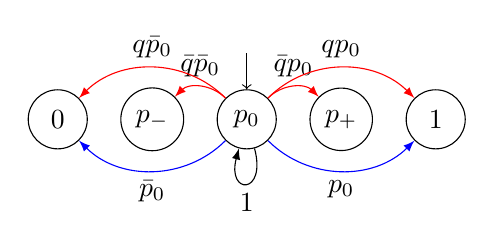
\begin{tikzpicture}
    \node[draw, minimum width=0.75cm, node distance=1.2cm, circle, initial above,initial text={} ] (bi) {$p_0$};
    \node[draw, minimum width=0.75cm, node distance=1.2cm, circle, left of=bi] (bm) {$p_-$};
    \node[draw, minimum width=0.75cm, node distance=1.2cm, circle, right of=bi] (bp) {$p_+$};
    \node[draw, minimum width=0.75cm, node distance=1.2cm, circle, right of=bp] (b1) {$1$};
    \node[draw, minimum width=0.75cm, node distance=1.2cm, circle, left of=bm] (b0) {$0$};

    \draw[-latex, red] (bi) to[out=45, in=135] node[black, above] {$\bar q p_0$} (bp);
    \draw[-latex, red] (bi) to[out=135, in=45] node[black, above] {$\bar q \bar p_0$} (bm);
    \draw[-latex, red] (bi) to[out=45, in=135] node[black, above] {$q p_0$} (b1);
    \draw[-latex, red] (bi) to[out=135, in=45] node[black, above] {$q \bar p_0$} (b0);
    \draw[-latex, blue] (bi) to[out=-45, in=-135]  node[black, below] {$p_0$} (b1);
    \draw[-latex, blue] (bi) to[out=-135, in=-45]  node[black, below] {$\bar p_0$} (b0);
    \draw[-latex, black] (bi) to[loop below] node[below, black] {1} (bi);
  \end{tikzpicture}
  \end{center}
  \caption{Illustration of environment belief model for a single region, only transitions from initial state $p_0$ are shown. Bars denote the complementary probability, i.e. $\bar p = 1-p$. When a high-quality measurement is received (blue edges), the belief transitions to $1$ with probability $p_0$ and to $0$ with probability $1-p_0$, whereas a low-quality measurement yields certainty with probability $q$ but with probability $1-q$ results in an intermediate belief $p_-$ or $p_+$. When no measurement is taken (black) the state does not change. The full transition matrices are given in}
  \label{fig:envmdp}
\end{figure}

We assume that regions of interest have been extracted from low-resolution satellite imagery, along with prior probability estimates for the likelihood that the regions exhibit certain traits. Here we restrict attention to \emph{risk regions} that may contain obstacles the rover can not traverse, and \emph{target regions} that are likely places where scientific samples can be extracted. We associate to each region $R$ a belief MDP $\MDP_{R}$ with five states $\zeta \in \{ 0, p_-, p_0, p_+, 1\}$ and three inputs $v \in \{ N, W, S \}$ for (N)o measurement, (W)eak measurement, and (S)trong measurement. The transition matrices are $T_N = I_5$, 
\begin{equation}
  T_{S} = \left[\begin{smallmatrix}
    1        &  0  &  0  &  0  &  0   \\
    \bar p_- &  0  &  0  &  0  &  p_- \\
    \bar p_0 &  0  &  0  &  0  &  p_0 \\
    \bar p_+ &  0  &  0  &  0  &  p_+ \\
    0        &  0  &  0  &  0  &  1
  \end{smallmatrix}\right],
  T_{W} = \left[\begin{smallmatrix}
    1        &  0                &  0  &  0           &  0   \\
    q\bar p_-&  \bar q \bar p_-  &  0  &  \bar q p_-  &  q p_- \\
    q\bar p_0&  \bar q \bar p_0  &  0  &  \bar q p_0  &  q p_0 \\
    q\bar p_+&  \bar q \bar p_+  &  0  &  \bar q p_+  &  q p_+ \\
    0        &  0  &  0  &  0  &  1
  \end{smallmatrix}\right].
\end{equation}
Here $q$ is a parameter denoting the quality of the weak measurement: if $q=0$ weak measurements are incapable of determining the true nature of the region, only intermediate beliefs $p_-$ and $p_+$ can be reached. For $q \in (0,1]$ there is a probability of a transition to a belief state 0 or 1. The outgoing transitions from $p_0$ are illustrated in Figure \ref{fig:envmdp}.

Given belief MDPs $\MDP_{R_i}$ for every region of interest, we construct the environment model $M_{env}$ as the parallel product
\begin{equation}
  \MDP_{env} = \MDP_{R_1} \otimes_{par} \MDP_{R_1}  \otimes_{par} \ldots \otimes_{par} \MDP_{R_n}. 
\end{equation}

\paragraph{Specification}

The objective of the mission is to satisfy a scLTL specification $\varphi$ over propositions over states in $\MDP_{rov}$ and $\MDP_{env}$. Examples of such propositions include
\begin{itemize}
  \item Don't enter a risk region $R_1$ that may contain an obstacle: $\xi_r \not  \in R_1 \lor \zeta_1 = 0$.
  \item Collect a sample at region $R_2$: $\xi_r \in R_2 \land \zeta_2 = 1$.
\end{itemize}

We posit that the rover has a time window of length $T_r$ to fulfill its mission, and that the copter has battery sufficient to operate for a time $T_c$. In addition, the copter must land in a pre-designated landing area $X_l$ at the end of the execution. This auxiliary objective is straightforward to incorporate into \eqref{eq:coptervalue} by restricting the value iteration to policies that land safely with some high probability $1-\delta_l$.

\paragraph{Measurement model}

We connect the systems in serial as illustrated in Fig \ref{fig:agg}. The serial products are defined via a connection maps that map the state of one system to the input of the next. These connections are defined as follows:
\begin{itemize}
  \item If the rover is adjacent to a region $R_i$ it takes a (S)trong measurement of that region,
  \item If the copter is at low altitude and in region $R_i$, it takes a (S)trong measurement of that region,
  \item If the copter is at high altitude and within distance $2$ of region $R_i$, it takes a (W)eak measurement of that region,
  \item The connection $C_\varphi$ defining the $\MDP_{rov} \otimes_{ser}^{C_\varphi} \MDP_{env}$ product is given by the truth value of atomic propositions for the state $(\xi_r, \xi_e)$.
\end{itemize}


\subsection{Illustrations}

We demonstrate the features of the proposed solution in a few example scenarios.

\paragraph{Scenario 1} If a sample of type $A$ exists, collect samples of types $A$ and $B$, otherwise collect a sample of type $C$, all while avoiding obstacles. Letting $\lozenge_o \varphi = \lnot \texttt{obstacle} \; \mathcal U \; \varphi$, the specification can be written
\begin{equation*}
  \left( \lozenge_o \texttt{sA} \land \lozenge_o \right) \texttt{sB} \lor \left( \lozenge_o ( \texttt{eA} \land \texttt{sC} ) \right).
\end{equation*}
The atomic propositions are defined as follows:
\begin{itemize}
	\item \texttt{sA} is $\True$ if $\xi_r \in A$ (rover is in region $A$) and $\zeta_A = 1$ (sample detected in $A$), and similarly for \texttt{sB} and \texttt{sC},
	\item \texttt{eA} is $\True$ if $\zeta_A = 0$ (there is no sample at $A$)
\end{itemize}
The workspace is shown in Figure \ref{fig:workspace1}; the prior probability estimates are $0.5$ for each region. We assume that the rover can move for $T_r = 15$ time steps, and that the copter has enough battery to move for $T_c - T_r = 30$ time steps (including changes of altitude). With the two-stage approach described in Section \ref{sec:solution} we can then compute 1) a value function $V_r(\xi_r, \xi_e, \xi_\varphi)$ and corresponding policy for the rover, and 2) a policy for the quadrotor that maximizes the probability of reaching a state where $V_r(\xi_r^0, \xi_e, \xi_\varphi^0)$ is either close to 0 or close to 1.

Executions generated from the resulting copter and rover policies are shown in Fig. \ref{fig:copter_executions} for different configurations of the true environment state. With only prior knowledge about the environment, the probability that the rover can satisfy the specification is $V_r(\xi_r^0, \xi_e^0, \xi_\varphi^0) = 0.25$. However, after the copter exploration all uncertainty is removed: for the two upper examples in Figure. \ref{fig:copter_executions}, $V_r(\xi_r^0, \xi_e^{T_{c}}, \xi_\varphi^0) = 1$ where $\xi_e^{T_c}$ is the environment belief state after copter exploration, and for the lower examples $V_r(\xi_r^0, \xi_e^{T_{c}}, \xi_\varphi^0) = 0$. This shows that the generated policy explores the environment in a way that efficiently reduces uncertainty about whether the specification can be satisfied.

\begin{figure}
  \begin{center}
    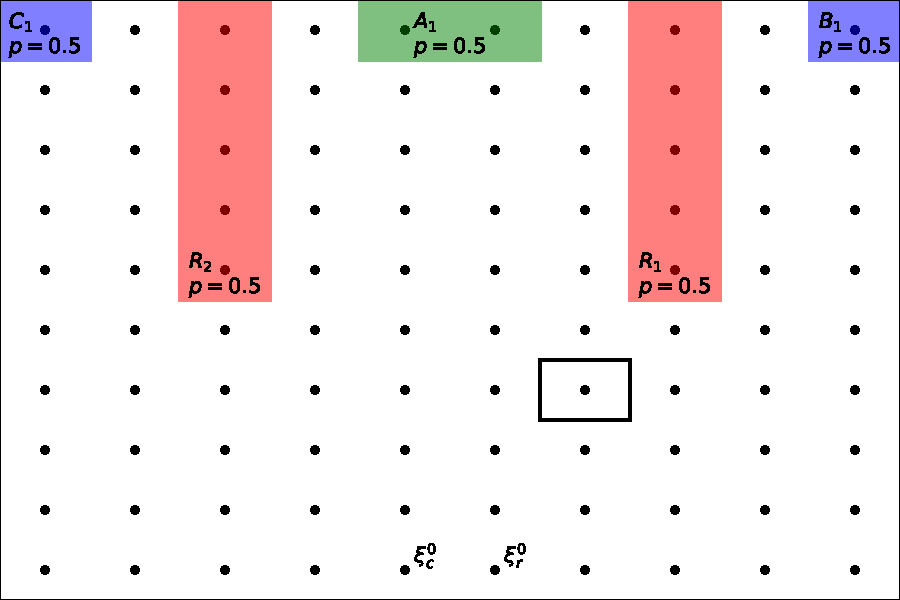
\includegraphics[width=0.6\columnwidth]{2figs/arena.pdf}
  \end{center}
  \caption{2D view of the work space where regions of interest $R_1$, $R_2$, $A$, $B$, and $C$ are marked along with associated prior probabilities. Each abstract state is illustrated with a dot. The black square marks the required landing zone for the copter.}
  \label{fig:workspace1}
\end{figure}

\todo{Connect this example with the Terraswarm example of Sheshia.}

\begin{figure}
	\begin{center}
	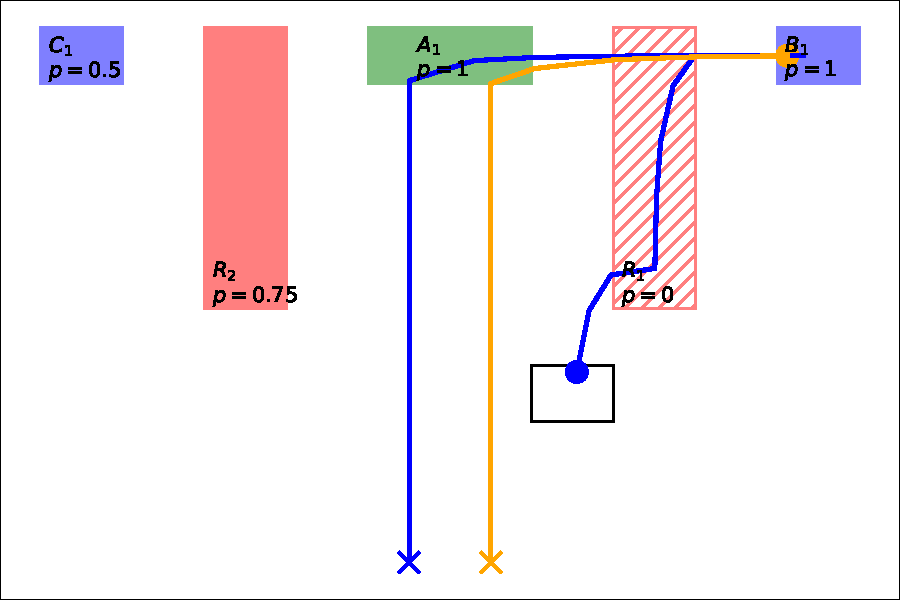
\includegraphics[width=0.4\columnwidth]{2figs/exp0-map.pdf} ~ 
	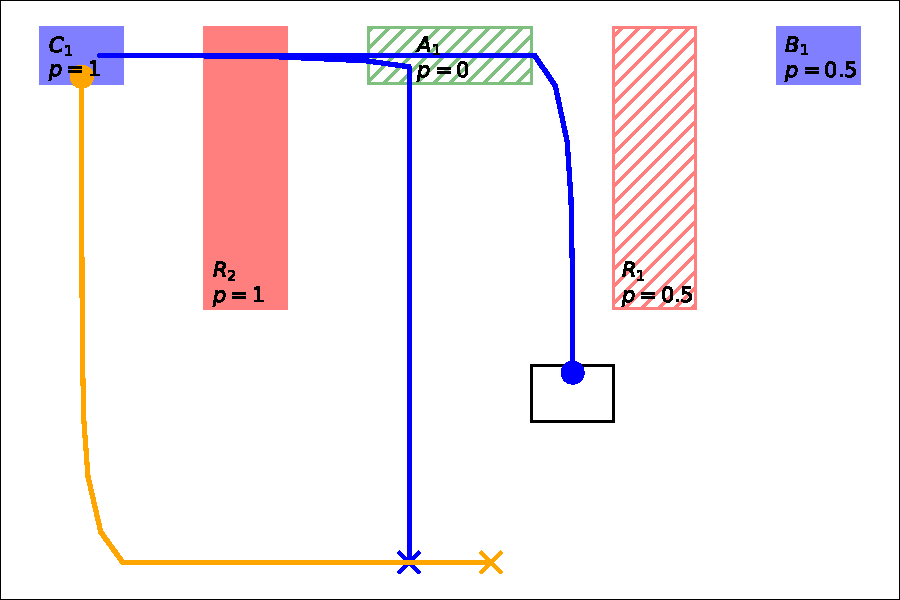
\includegraphics[width=0.4\columnwidth]{2figs/exp1-map.pdf} \\
	\vspace{1mm} 
	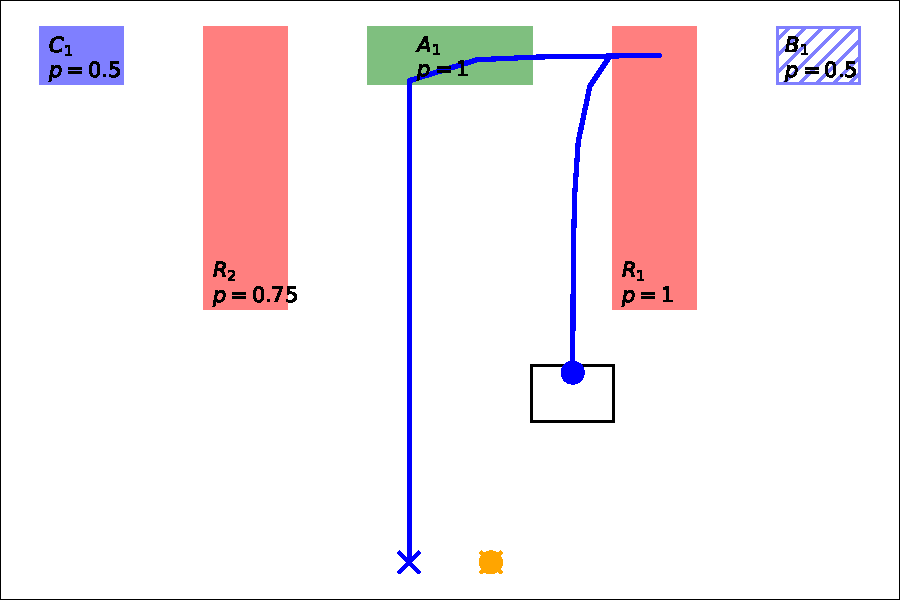
\includegraphics[width=0.4\columnwidth]{2figs/exp2-map.pdf} ~ 
	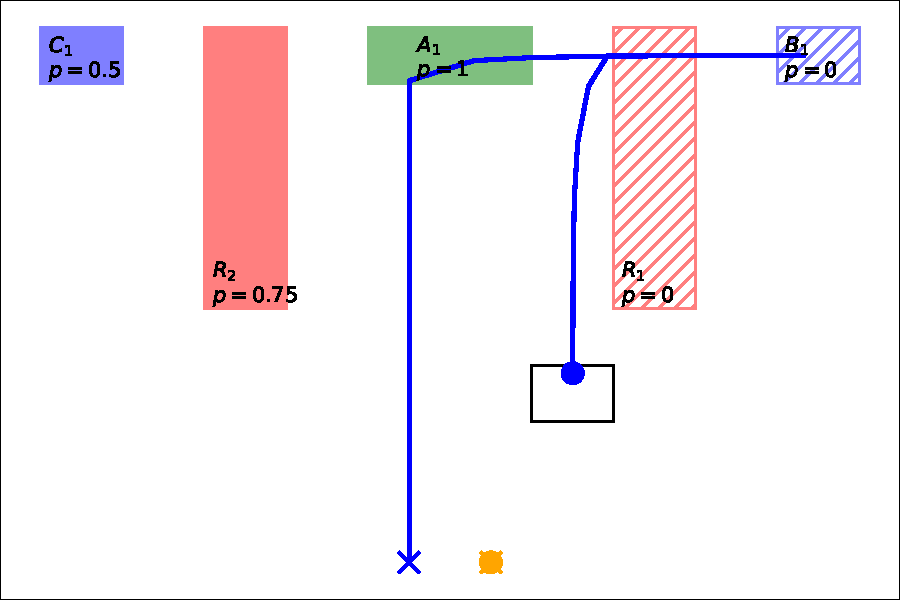
\includegraphics[width=0.4\columnwidth]{2figs/exp3-map.pdf}
	\end{center}
	\caption{Illustration of the copter and rover policies for different environment configurations: a shaded region indicates that the true state is equal to 0 (i.e. no sample or obstacle). The region probabilities indicate the belief states after the copter exploration phase. Copter trajectories are shown in blue, and rover trajectories in orange, if the specification can not be satisfied the rover does not move. All four executions are generated by the exact same policies; they adapt according to measurements received during the execution.\sofie{can you also differentiate height of the copter. Picture is not black/white proof. } }
	\label{fig:copter_executions}
\end{figure}

% \begin{figure}
%   \begin{center}
%     \footnotesize
%     \begin{tikzpicture}
%       \node[inner sep=0] (p1) {
\includegraphics[height=0.24\columnwidth]{2figs/value-rov.pdf}};
%       \node[inner sep=0, anchor=west] at ([xshift=2mm]$(p1.east)$) (p2) {
\includegraphics[height=0.24\columnwidth]{2figs/value-cop.pdf}};
%       \node[inner sep=0, anchor=west] at ([xshift=2mm]$(p2.east)$) (n1) {
\includegraphics[height=0.24\columnwidth]{2figs/cbar.pdf}};
%       \node at ([yshift=2mm]$(p1.north)$) {$V_0^1(\xi_r, \xi_e^0, \xi_\varphi^0)$};
%       \node at ([yshift=2mm]$(p2.north)$) {$V_0^2(\xi_c, \xi_e^0)$};
%       \node at ([xshift=6mm]$(n1.north east)$) {$p = 0.48$};
%       \node at ([xshift=6mm]$(n1.south east)$) {$p = 0$};
%     \end{tikzpicture}
%   \end{center}
%   \caption{Illustration of value functions. As can be seen, the advantage of the copter is equivalent to having the rover's initial state be near a target region.}
%   \label{fig:values1}
% \end{figure}

\section{Hardware Experiments}
\label{sec:hardware}

\begin{itemize}
    \item Copter in CAST
\end{itemize}


\section{Conclusion}
\label{sec:conclusion}

\begin{itemize}
	\item Point out that approach is compatible with label-based abstractions
\end{itemize}

Future work:
\begin{itemize}
	\item Improved scalability via approximate DP, sparse value function representations (forego exactness)
	\item Our solution method is however agnostic to the model components; they could substituted for models obtained from formal abstraction procedures or from sampling-based methods. 
\end{itemize}


\printbibliography

\end{document}

